This section presents a detailed overview of the program flow of the final interrupt-oriented paddle program, relying heavily on UML flow diagrams to convey the program structure.

The entire program follows the classic init-loop structure, as pictured in figure \ref{fig:main-program-flow}. Note that there is no deinit code, as the program is intended to run forever in an environment without an operating system.

The rest of the program is mainly subroutine-based, making use of labels as subroutine names, and returning values with the \texttt{ret} instruction. This allows for relatively modular and readable code, which is a challenge in general, but especially much so when writing in assembly.

\begin{figure}
\includegraphics[width = \textwidth]{description-and-methodology/program-flow/main-program-flow.pdf}
\caption{Main superficial program flow}
\label{fig:main-program-flow}
\end{figure}

Figure \ref{fig:init} details the init section of the program.

\begin{figure}
\includegraphics[width = \textwidth]{description-and-methodology/program-flow/init.pdf}
\caption{Initialization}
\label{fig:init}
\end{figure}

Figure \ref{fig:main-loop} details the main loop of the program. From this main loop, many sub-routines are called. These sub-routines are detailed in figures \ref{fig:set-leds}, \ref{fig:move-paddle-right}, and \ref{fig:move-paddle-left}.

\begin{figure}
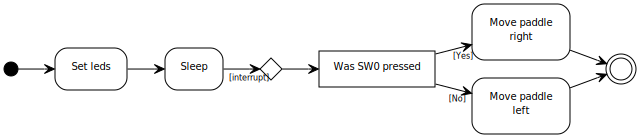
\includegraphics[width = \textwidth]{description-and-methodology/program-flow/main-loop.pdf}
\caption{Main loop}
\label{fig:main-loop}
\end{figure}

\begin{figure}
\includegraphics[width = \textwidth]{description-and-methodology/program-flow/set-leds.pdf}
\caption{Set leds subroutine}
\label{fig:set-leds}
\end{figure}

\begin{figure}
\includegraphics[width = \textwidth]{description-and-methodology/program-flow/button-interrupt-routine.pdf}
\caption{Button interrupt routine}
\label{fig:button-interrupt-routine}
\end{figure}

At any time, a button interrupt may occur, at which time the button interrupt routine is called.
The button interrupt routine is detailed in figure \ref{fig:button-interrupt-routine}.
The button interrupt routine calls the subroutines \texttt{read\_buttons} (figure \ref{fig:read-buttons}), and \texttt{debounce} (figure \ref{fig:debounce}).

\begin{figure}
\includegraphics[width = \textwidth]{description-and-methodology/program-flow/debounce.pdf}
\caption{Debounce subroutine}
\label{fig:debounce}
\end{figure}

\begin{figure}
\includegraphics[width = \textwidth]{description-and-methodology/program-flow/read-buttons.pdf}
\caption{Read buttons subroutine}
\label{fig:read-buttons}
\end{figure}

\begin{figure}
\includegraphics[width = \textwidth]{description-and-methodology/program-flow/move-paddle-right.pdf}
\caption{Move paddle right subroutine}
\label{fig:move-paddle-right}
\end{figure}

\begin{figure}
\includegraphics[width = \textwidth]{description-and-methodology/program-flow/move-paddle-left.pdf}
\caption{Move paddle left subroutine (analogous to move paddle right subroutine, but included for completeness)}
\label{fig:move-paddle-left}
\end{figure}

